\section{Product Environment}

\subsection{Software}
\begin{frame}{ROOT}
    \begin{itemize}
      \item process and visualize large amounts of scientific data (CERN)
      \item features a C++ interpreter (CLING) - i.e. used for rapid and efficient prototyping
      \item persistency mechanism for C++ objects
    \end{itemize}

    % \pause \kitbottom

  \begin{figure}[htb]
    \centering
    \begin{subfigure}[b]{0.5\textwidth}
           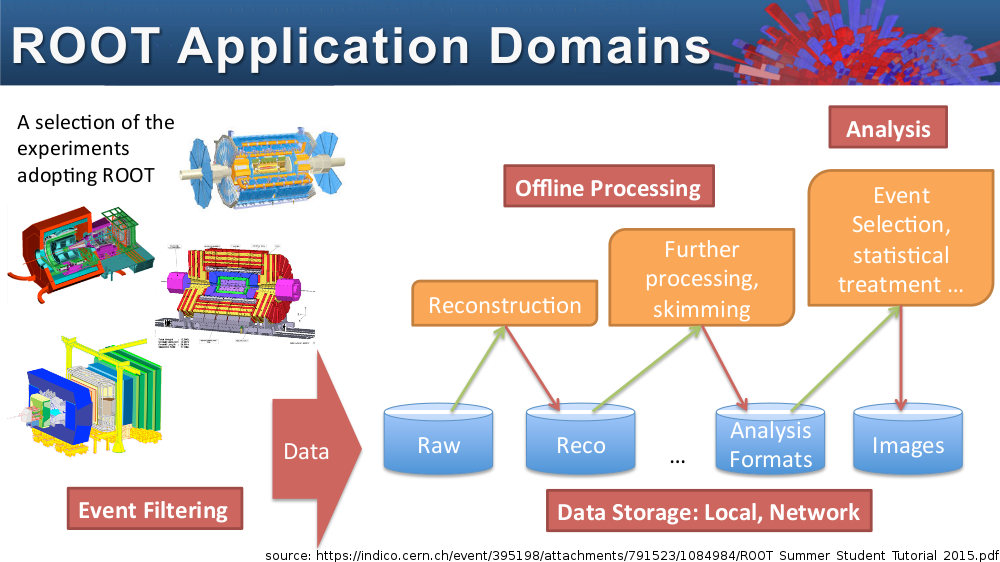
\includegraphics[width=0.97\linewidth, keepaspectratio]{./resources/root_application_domains.png}
           \nocite{cern:tut}
           %\caption{My Caption\footnotemark}
    \end{subfigure}%
    \begin{subfigure}[b]{0.5\textwidth}
          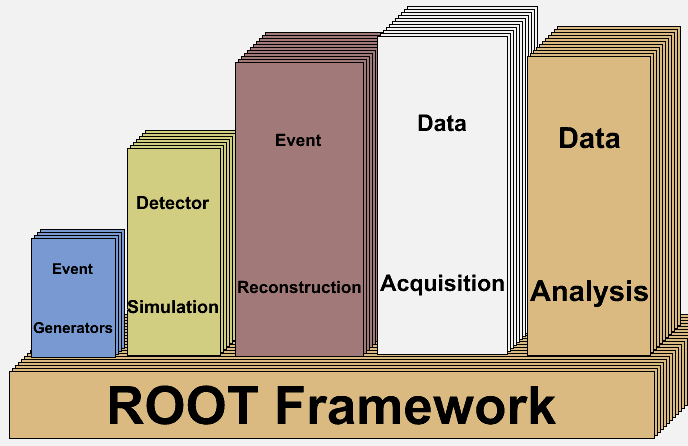
\includegraphics[width=0.97\linewidth, keepaspectratio]{./resources/root_application_domains2.png}
          \nocite{cern:domains}
    \end{subfigure}
  \end{figure}
  %\footnotetext{\cite{root_tut}}.}
\end{frame}

\begin{frame}{Node.js}

  \begin{itemize}
    \item open source runtime environment
    \begin{itemize}
        \item develop server side web applications
        \item act as a stand alone web server
    \end{itemize}

    \uncover<2->{
      \item Google V8 engine to execute JavaScript code
      \item rootJS bindings realized as native Node.js module written in C++
    }
  \end{itemize}

  \begin{figure}[htb]
    \centering
    
\includegraphics[width=0.97\linewidth, keepaspectratio]{./resources/nodejs-light.eps}
    \nocite{nodejs:logo}
  \end{figure}

\end{frame}

\subsection{Hardware}
\begin{frame}{Hardware}

\end{frame}
